\graphicspath{{images/}}

\subsection{Численные методы решения многомерных задач математической физики}

\subsubsection{Постановка задачи}
Используя схемы переменных направлений и дробных шагов, решить двумерную начально-краевую задачу для дифференциального уравнения параболического типа. В различные моменты времени вычислить погрешность численного решения путем сравнения результатов с приведенным в задании аналитическим решением $U(x, t)$. Исследовать зависимость погрешности от сеточных параметров $\tau$, $h_x$, $h_y$.

\subsubsection{Вариант 9}
$$ {{\partial u} \over {\partial t}} = a \cdot {{\partial^2 u} \over {\partial x^2}} + b \cdot {{\partial^2 u} \over {\partial y^2}} + \sin{x} \cdot \sin{y} \cdot (\mu \cdot \cos(\mu t) + (a + b) \cdot \sin(\mu t)) $$
\begin{itemize}
    \item $a = 1$, $b = 1$, $\mu = 1$;
    \item $a = 2$, $b = 1$, $\mu = 1$;
    \item $a = 1$, $b = 2$, $\mu = 1$;
    \item $a = 1$, $b = 1$, $\mu = 2$.
\end{itemize}
$$ u(0, y, t) = 0 $$
$$ u({{\pi} \over {2}}, y, t) = \sin{y} \cdot \sin(\mu t) $$
$$ u(x, 0, t) = 0 $$
$$ u(x, \pi, t) = -\sin{x} \cdot \sin(\mu t) $$
$$ u(x, y, 0) = 0$$
Аналитическое решение:
$$ U(x, y, t) = \sin{x} \cdot \sin{y} \cdot \sin(\mu t) $$
\pagebreak

\subsubsection{Результат}
\begin{center}
    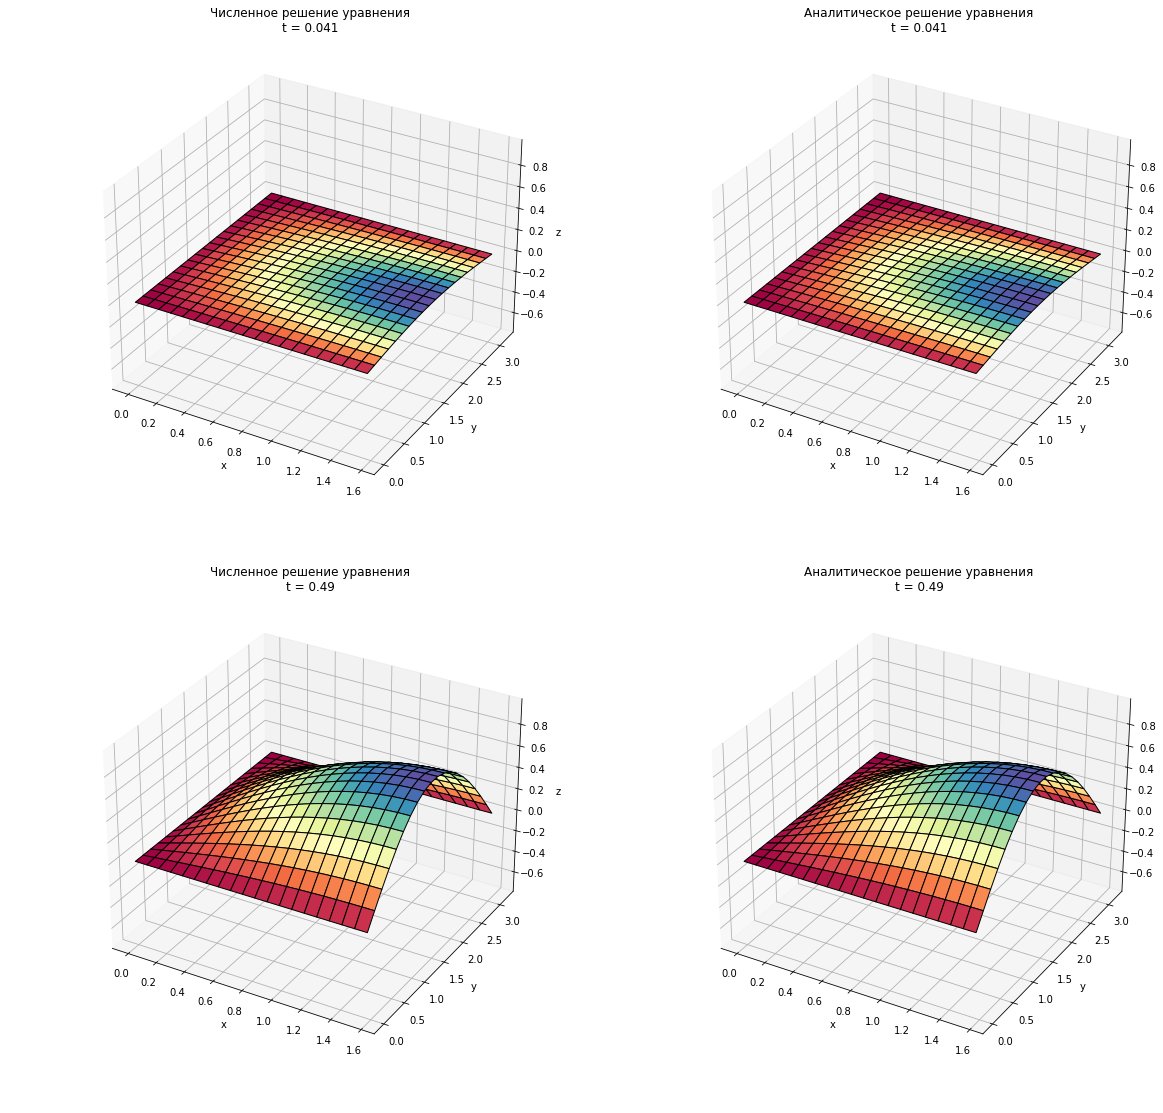
\includegraphics[width=\textwidth]{8_1.png}\newline\noindent
\end{center}
\pagebreak

\begin{center}
    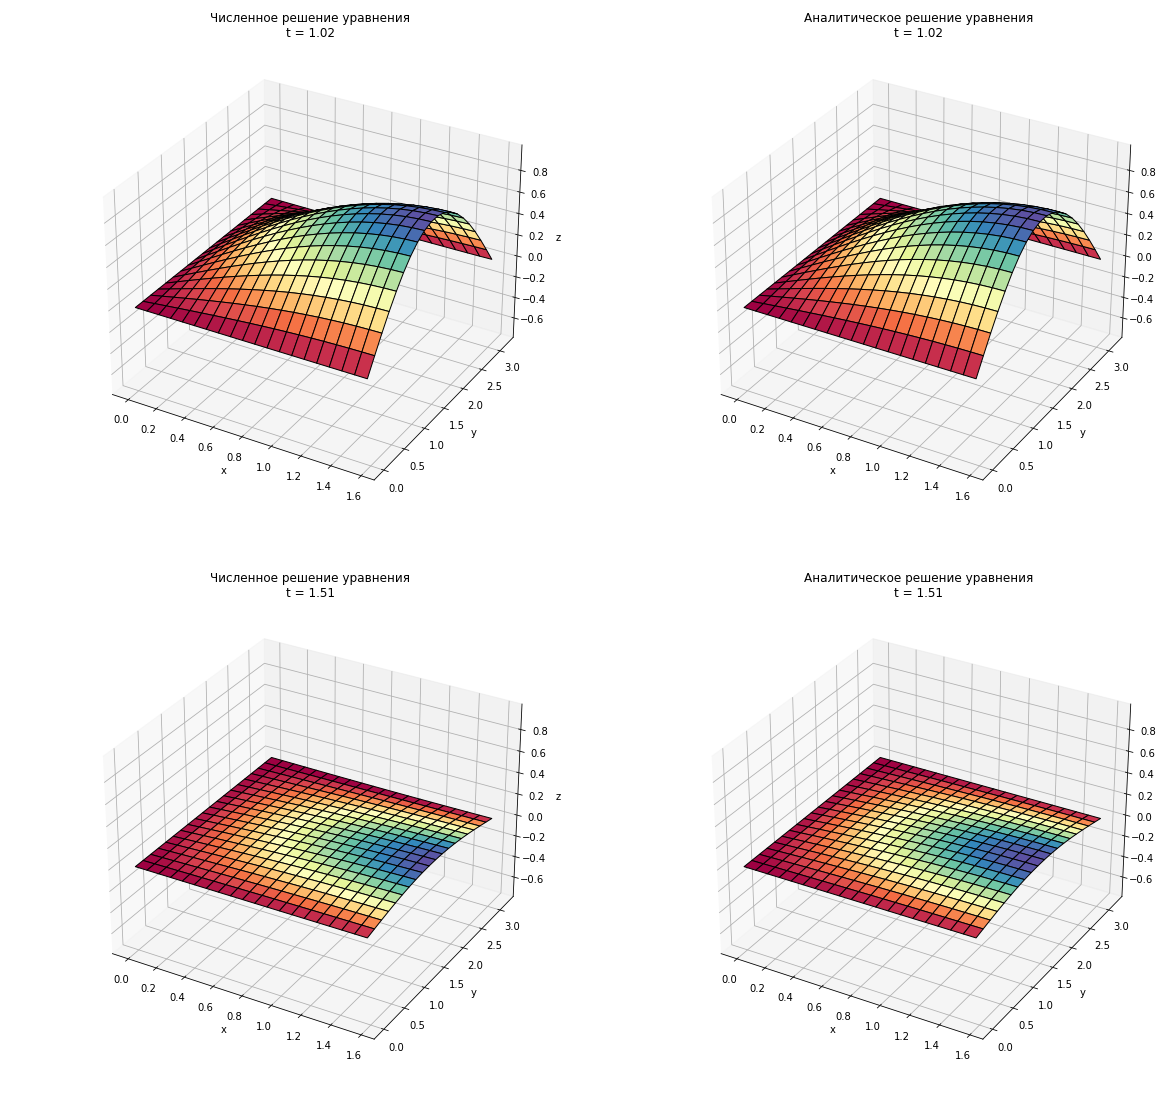
\includegraphics[width=\textwidth]{8_2.png}\newline\noindent
\end{center}
\pagebreak

\begin{center}
    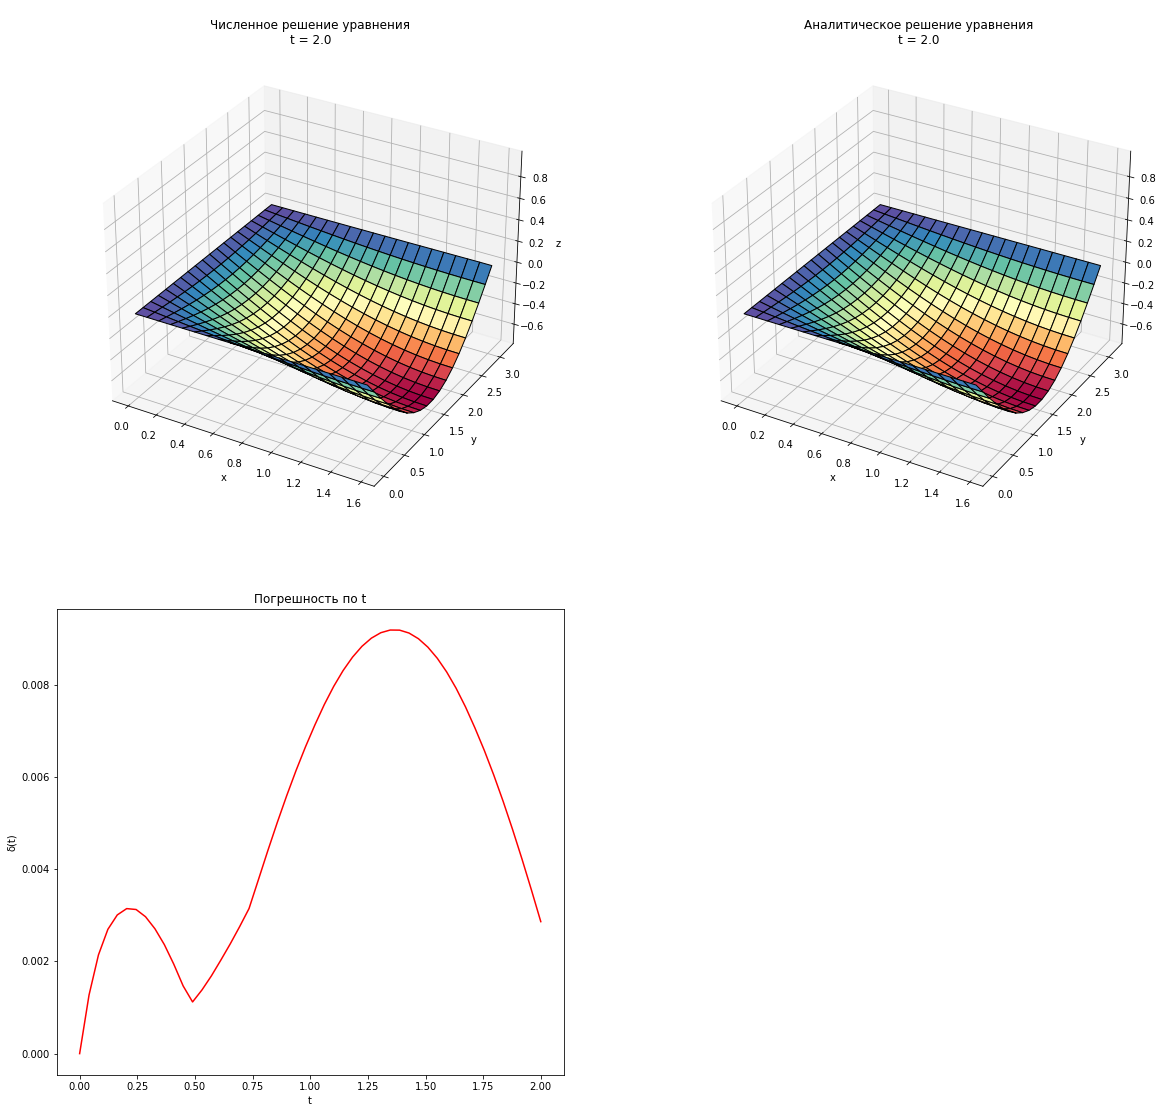
\includegraphics[width=\textwidth]{8_3.png}\newline\noindent
\end{center}
\pagebreak

\subsubsection{Исходный код}
\lstinputlisting{../lab8/ppde2d.hpp}
\pagebreak
